The first attempts to mathematically characterize musical intervals date back to Pythagoras, who noted that the consonance of two tones played on a monochord can be related to simple fractions of the corresponding string lengths (for a general introduction see e.g. \cite{Geller,White}). Physically this phenomenon is caused by the circumstance that oscillators such as strings do not only emit their fundamental ground frequency but also a whole series of partials (overtones) with integer multiples of the ground frequency. Consonance is related to the accordance of higher partials, i.e., two tones with fundamental frequencies $f$ and~$f'$ tend to be perceived as consonant if the $m$-th partial of the first one matches with the $n$-th partial of the second, meaning that $mf=nf'$ (see Fig. \ref{spectra}). Although the perception consonance is a highly complex psychoacoustic phenomenon (see e.g.~\cite{mcdermott,stolzenburg}) which also depends on the specific context~\cite{milne,parncutt}, one can basically assume that the impression of consonance is particularly pronounced if $m$ and $n$ are small. Examples include the perfect octave $(m/n=2/1)$, the perfect fifth ($3/2$), and the perfect fourth ($4/3$). Larger values of $m$ and $n$ tend to correspond to more dissonant intervals. If a normally consonant interval is sufficiently detuned from the ``just'' tuning, i.e., the simple frequency ratio, the resulting mismatch of almost-coinciding partials leads to a superposition of waves with slightly different frequencies~\cite{helmholtz}. The fast beating of these almost-coinciding partials can result in a sensation of roughness or being out of tune that ruins the perception of consonance.

%------------------------------------------------------------------------
\begin{figure}[t]
\centering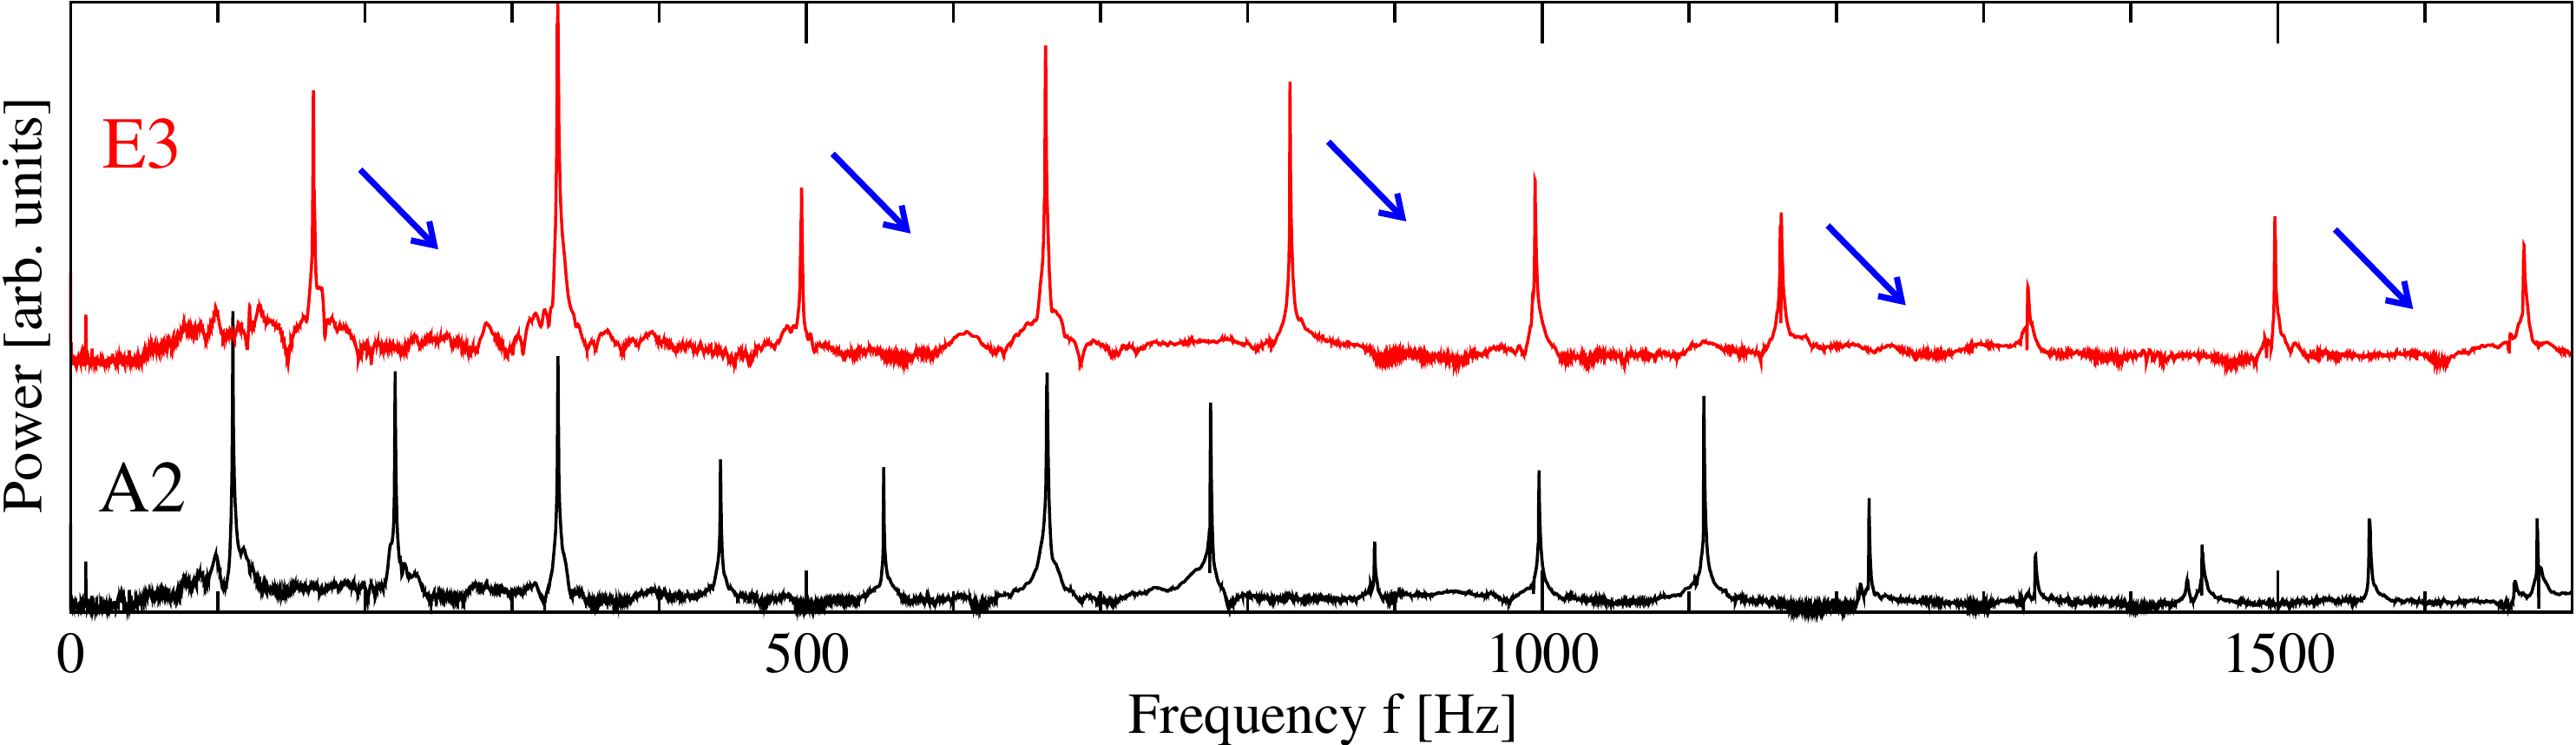
\includegraphics[width=150mm]{spectra}
\caption{Consonance of a just perfect fifth. The figure shows a measured power spectrum of the piano keys A2 (110 Hz) and E3 (165 Hz). As first theorized by Helmholtz (1877)~\cite{helmholtz}, the fifth is perceived as consonant because many partials of the corresponding natural harmonic series coincide (marked by the arrows in the figure).\label{spectra}}
\end{figure}
%------------------------------------------------------------------------

With the historical development of fretted instruments and keyboards, it made sense to define a system of fixed frequencies in an octave-repeating pattern. The frequency ratios of stacked intervals multiply. (For example, the chord A2-E3-B3, consisting of two perfect fifths each having the ratio $3/2$, yields a frequency ratio of $9/4$ from A2 to B3.) This immediately confronts us with the fundamental mathematical problem that multiplication and prime numbers are incommensurate in the sense that powers of prime numbers never yield other simple prime numbers. For example, it is impossible to match $k$ just perfect fifths with $\ell$ just octaves since $(3/2)^k \neq (2/1)^\ell$ for all $k,\ell\in \mathbb{N}$. Mathematically speaking, the concatenation of just musical intervals (by multiplying their frequency ratios) is an operation that does not close up on any finite set of tones per octave.

Fortunately the circle of fifths approaches a closure up to a small mismatch: when stacking twelve just fifths on top of each other the resulting frequency ratio $(3/2)^{12}$ differs from seven octaves (ratio $2^7$) only by a small amount; explaining why the Western chromatic scale is based on twelve semitones per octave. Nevertheless the remaining difference of $\approx 1.4\%$ ($23.46$ cents\footnote{In music theory, a cent ($\cent$) is defined as 1/100 of a semitone in the equal temperament.}), known as the Pythagorean comma, is clearly audible and cannot be neglected in a scale with fixed frequencies.  Likewise, a sequence of four just fifths transposed back by two octaves ($(3/2)^4/2^2$) differs from a major third of $5/4$ by the so-called syntonic comma of $21.51$ cents.

Since it is impossible to construct a musical scale that is based exclusively on pure beatless intervals, one has to seek out suitable compromises. Over the centuries this has led to a fascinating variety of tuning systems, called temperaments, which reflect the harmonic texture of the music in the respective epoch~\cite{Barbour}. With the increasing demand of flexibility the equal temperament (ET) finally prevailed in the 19$^{\rm th}$ century and has established itself as a standard temperament of Western music. In the ET the octave is divided into twelve equally sized semitones of constant frequency ratio $2^{1/12}$. The homogeneous geometric structure of the ET ensures that all interval sizes are invariant under transposition (displacements on the keyboard). This means that music can be played in any key, differing only in the global pitch but not in the harmonic texture. 

However, this high degree of symmetry can only be established at the expense of harmony~\cite{DuffinBook}. In fact, the only just interval in the ET is the octave with the frequency ratio $2/1$ while all other intervals are characterized by irrational frequency ratios, deviating from the just intervals. For some intervals the variation is quite small and hardly audible, e.g., the equally tempered fifth differs from the just perfect fifth by only two cents. For other intervals, however, the deviations are clearly audible if not even disturbing. For example, the minor third in the ET is almost $16\cent$ smaller than the natural frequency ratio 6:5. The same applies to the major third which is about $14\cent$ greater than the ratio 5:4. These discrepancies may explain why there was some reluctance among many musicians to accept the ET. It was not until the 19th century that the ET became a new tuning standard, presumably both because of Western music's increasingly complex harmonies and because of an increasing intonational tolerance on the part of the audience.\\

\noindent\textbf{Just Intonation}
~\newline~\newline
Although musical temperaments provided a good solution for most purposes, music theorists and instrument makers have searched for centuries for possible ways to overcome the shortcomings of temperaments, aiming to play music solely on the basis of pure intervals, referred to as \textit{just intonation} (JI)~\cite{DuffinArticle}. Tuning an instrument in just intonation means to adjust the twelve pitches of the octave in such a way that all frequency ratios with respect to a certain reference frequency $f^*$ are given by simple rational numbers. For example, a possible choice of such frequency ratios is listed in Table~\ref{tab:frequencyratios}.

\begin{table}
\begin{center}
\begin{tabular}{l|cccccccccccc}
semitones& 0 & 1 & 2 & 3 & 4 & 5 & 6 & 7 & 8 & 9 & 10 & 11\\ \hline
$f/f^*$ & 1 & 16/15 & 9/8 & 6/5 & 5/4 & 4/3 & 45/32 & 3/2 & 8/5 & 5/3 & 9/5 & 15/8 
\end{tabular}
\end{center}
\caption{The most common choice of frequency ratios in just intonation, known 5-limit tuning. }
\label{tab:frequencyratios}
\end{table}

Just intonation always refers to the tonic of a given scale, referred to in this article as the \textit{keynote}. In its own reference scale, JI sounds very consonant if not even sterile, but unfortunately a transposition in other scales is not possible. For example, tuning a piano in just intonation with keynote C,  a C-major triad sounds consonant while most triads in other keys appear to be out of tune. The same applies to modulations from one key to another. Thus, for good reasons, just intonation has the reputation of being absolutely impractical.

To overcome this problem, a possible solution would be to enlarge the number of tones per octave. Important historical examples are for example a keyboard with 19 keys per octave suggested by the renaissance music theorist G. Zarlino (1558), and the two-manual archichembalo by N. Vicentino (1555) with 36 keys per octave~\cite{Vicentino}. More recent examples include the Bosanquet organ with 48 keys per octave (see~\cite{helmholtz}), the harmonium with 72 keys per ocatave by~\cite{Oettingen}, and the 31-tone organ by~\cite{fokker}. Today various types of electronic microtonal interfaces are available~(see \cite{Douglas,macritchie}). However, as one can imagine, such instruments are very difficult to play.

\vspace{2mm}
Temperaments are primarily relevant for keyboard instruments (such as piano, harp, organ) and fretted instruments (e.g. lute and guitar), where all tones are tuned statically in advance. In comparison many other instruments (e.g. string instruments) allow the musician to recalibrate the pitches during the performance, and the same applies of course to the human voice. Musicians playing such instruments tune the pitches \textit{dynamically} while the music is being played. By listening to the harmonic consonance and its progression, well-trained musicians are able to estimate the appropriate frequency intuitively and to correct their own pitch instantaneously. Usually the played notes are a compromise between just intervals and the prevailing ET~\cite{DuffinArticle}. By dynamically adapting the pitches, this allows one to significantly improve the harmonic texture. In this respect the following quotation of the famous cellist Pablo Casals~\cite{Casals} seems to make a lot of sense: 
\begin{quote}
\textit{``Don’t be scared if your intonation differs from that of the piano. It is the piano that  is out of tune.  The piano with its tempered scale is a compromise in intonation.''} 
\end{quote}
\vspace{2mm}

\noindent\textbf{Dynamically Adapting Tuning Schemes}
~\newline~\newline
Is it possible to mimic the process of dynamical tuning by constructing a device which instantaneously calculates and corrects the pitches like a singer in a choir? This idea can be traced back to the early days of electronic keyboard instruments. Since then various implementations have been suggested, the most important ones including \textit{GrovenMax}~\cite{GrovenMax}, \textit{Justonic Pitch Palette}\texttrademark~\cite{Justonic}, \textit{Mutabor}~\cite{Mutabor}, \textit{Hermode Tuning}\texttrademark~\cite{Hermode}, and \textit{TransFormSynth}~\cite{Sethares}. These will be described in the following.

\begin{itemize}
\item One of the first pioneers of dynamic tuning schemes was the Norwegian microtonal composer and music-theorist Eivind Groven~\cite{GrovenMax}. In 1936 he constructed a pipe organ driven by an electric circuit of relays used in telephone switchboards at that time.The organ had three sets of pipes differing by a syntonic comma. Playing a chord on the manual, the electro-mechanical logical circuit computed the optimal arrangement of the chord and triggered the pipes accordingly. In 1995 this method was implemented on a computer, redirecting the output of a MIDI keyboard to three MIDI pianos differing in pitch by a syntonic comma~\cite{Premiere}.

\item\textit{Justonic Pitch Palette}\texttrademark ~was proprietary software produced by Justonic Tuning, Inc. based on a patented method developed by J. William Gannon and Rex A. Weyler~\cite{Justonic}. This tuning method is dynamic in so far as the artist himself can change the keynote frequency $f^*$ during the performance by hand. The corresponding frequencies are then retrieved from a table and sent to a microtonal synthesizer. The selection of the keynote requires additional hardware such as an extra manual.

\item\textit{Mutabor} is a microtonal software project initiated by M. Vogel at the University of Darmstadt~\cite{Mutabor}. The first version, referred to as Mutabor I, was designed as ``\textit{a system with 171 steps per octave for electronic keyboard instruments}''. Depending on the actual chord being played, the program calculates the actual chordal root and tries to tune all frequencies in pure fifths, fourths, and thirds. However, this leads to audible frequency shifts between subsequent chords. From 1987 on Mutabor II improved this method, aiming to produce a usable PC-software for MIDI devices and allowing the user to develop individual tuning algorithms. In a third stage starting in 2006, Mutabor has evolved into a full-fledged microtonal programming language. Nevertheless, for music with a greater harmonic complexity, the chordal root is not always detected reliably. As a solution, Mutabor offers the user to pre-determine the succession of keynotes in a separate MIDI file.

\item \textit{Hermode Tuning}\texttrademark ~is a commercial adaptive tuning scheme developed by Werner Mohrlok~\cite{Hermode}. To our knowledge it is the only adaptive tuning scheme that has reached a wider dissemination, ranging from implementations in church organs to plugins for software packages such as \textit{Cubase}\texttrademark. Instead of determining the chordal root, the algorithm tunes intervals between adjacent tones of a given chord instantly to just ratios. At the same time the global pitch is adjusted in such a way that the difference to the usual ET is minimized. This reduces the disturbing frequency shifts between subsequent chords. Hermode tuning also tries to compensate the so-called pitch drift (see section \ref{PitchDrift}).

\item\textit{TransFormSynth} is a freely available software-based synthesizer developed by William A. Sethares~\cite{Sethares}. Unlike all other approaches -- including the one presented here -- which are based on the idea of dynamically modifying the fundamental frequencies and thereby the whole series of corresponding partials, Sethares  proposes to keep the fundamental frequencies fixed (e.g. according to the ET). Instead, his algorithm modifies the frequencies of the higher partials in such a way that they match. As a result, even though the overtone spectra are distorted, the synthesized sound nevertheless tends to be perceived as consonant\footnote{A similar phenomenon occurs in the context of piano tuning. Since the overtone spectra of stiff steel strings are slightly inharmonic, piano tuners stretch the tuning in order to compensate these deviations.}. As far as we can see, this method is restricted to synthesizers which allow the overtone spectra to be specified individually, but it cannot be applied to ordinary musical instruments with natural harmonic overtone spectra.
\end{itemize}

\noindent
All these methods except for the last one are similar in that they analyze a given chord and then make decisions for tuning the frequencies, i.e. they are defined in procedural terms. Depending on the harmonic context, these decisions can be quite complex with different possible solutions for the same situation.

In the present paper, we investigate an alternative adaptive tuning scheme based on a different method which was originally proposed by~\cite{Laubenfels} (unpublished, for a short summary see~\cite{Sethares2005}). Instead of making a sequence of \textit{if-then} decisions, this method is defined mathematically and amounts to continuously solving a system of linear equations. As is described below, the system of equations may be viewed as a resistor network or likewise as a mechanical network of springs representing the interval sizes. Roughly speaking, each spring prefers to relax into a state where its length corresponds to the natural size of a pure interval and it will do so whenever this is possible, producing a chord in just intonation. However, if the spring network is so complex that it is impossible for all springs to simultaneously be situated in their ground state, the system will approach a non-trivial state under tension, representing a tempered harmonic compromise. This happens automatically without making any explicit decisions and may resemble the way in which musicians find the best possible intonation. As another advantage, the present method finds a harmonic compromise for \textit{all} intervals in a given chord, not only of the intervals between adjacent tones. 

To demonstrate the technical feasibility of the dynamically adjusting tuning scheme discussed in this paper, we implemented the tuning algorithm in an open-source application which is available for various platforms including mobile devices. This software will be described in more detail at the end of the paper.
